% OCR draft from PDF page 30. Needs cleanup and verification.
\chapter{Introduction}
\label{chap:introduction}

\section{Overview}
\label{sec:intro-overview}

This chapter introduces the simulation concepts and notation used throughout
the book. The following figures show the distribution of file lengths and an
example of sampling from that distribution.

\begin{figure}[htbp]
  \centering
  % Figure 1.1 (left): boxed table of file-length distribution.
  \begin{minipage}{0.38\textwidth}
    \centering
    \renewcommand{\arraystretch}{0.95}
    \fbox{%
      \begin{tabular}{c c}
        \textbf{length in} & \textbf{proportion} \\
        \underline{\textbf{tracks}} & \underline{\textbf{of files}} \\
        1  & .060 \\
        2  & .170 \\
        3  & .238 \\
        4  & .223 \\
        5  & .156 \\
        6  & .087 \\
        7  & .040 \\
        8  & .016 \\
        9  & .007 \\
        10 & .003 \\
      \end{tabular}%
    }
  \end{minipage}\hfill
  % Figure 1.1 (right): histogram with hatched bars.
  \begin{minipage}{0.52\textwidth}
    \centering
    \begin{tikzpicture}
      \begin{axis}[
        width=\textwidth,
        height=0.72\textwidth,
        ymin=0,
        ymax=0.25,
        xmin=0.3,
        xmax=10.7,
        ytick={.00,.05,.10,.15,.20,.25},
        yticklabels={\axisfont .00,\axisfont .05,\axisfont .10,\axisfont .15,\axisfont .20,\axisfont .25},
        xtick={1,2,3,4,5,6,7,8,9,10},
        xticklabels={\axisfont 1,\axisfont 2,\axisfont 3,\axisfont 4,\axisfont 5,\axisfont 6,\axisfont 7,\axisfont 8,\axisfont 9,\axisfont 10},
        tick label style={font=\axisfont\small,/pgf/number format/assume math mode=false},
        xticklabel style={font=\axisfont\small,/pgf/number format/assume math mode=false},
        yticklabel style={font=\axisfont\small,/pgf/number format/fixed,/pgf/number format/assume math mode=false},
        axis lines=box,
        axis line style={line width=2.2pt},
        tick style={black,line width=1pt},
        major tick length=6pt,
        minor tick length=3pt,
        minor y tick num=1,
        tick align=outside,
        xtick pos=left,
        ytick pos=left,
        enlargelimits=false,
        ymajorgrids=false,
        xmajorgrids=false,
      ]
        % Figure 1.1 histogram: horizontal dashed guides at selected heights.
        \addplot[black!50, dashed, line width=0.6pt, forget plot] coordinates {(0.5,0.060) (10.5,0.060)};
        \addplot[black!50, dashed, line width=0.6pt, forget plot] coordinates {(0.5,0.170) (10.5,0.170)};
        \addplot[black!50, dashed, line width=0.6pt, forget plot] coordinates {(0.5,0.238) (10.5,0.238)};
        \addplot[black!50, dashed, line width=0.6pt, forget plot] coordinates {(0.5,0.223) (10.5,0.223)};
        \addplot[black!50, dashed, line width=0.6pt, forget plot] coordinates {(0.5,0.156) (10.5,0.156)};
        \addplot[black!50, dashed, line width=0.6pt, forget plot] coordinates {(0.5,0.087) (10.5,0.087)};
        \addplot[
          ybar,
          bar width=0.081\textwidth,
          fill=white,
          draw=black,
          pattern={Lines[angle=45,distance=3pt,line width=0.7pt]},
          line width=3pt
        ]
          coordinates {
            (1,.060) (2,.170) (3,.238) (4,.223) (5,.156)
            (6,.087) (7,.040) (8,.016) (9,.007) (10,.003)
          };
      \end{axis}
    \end{tikzpicture}
  \end{minipage}
  \caption{Distribution of File Lengths}
  \label{fig:file-lengths}
\end{figure}

\begin{figure}[htbp]
  \centering
  % Figure 1.2 (left): uniform random variate scale + arrow.
  \begin{minipage}{0.3\textwidth}
    \hspace*{0.6cm}
    \pgfmathsetlengthmacro{\figtwoheight}{0.72\textwidth}
    \begin{tikzpicture}[x=1cm,y=\figtwoheight/5]
      \draw[->,line width=1pt] (0,0) -- (0,5);
      \foreach \y in {0,1,2,3,4} {
        \draw[line width=0.8pt] (-0.15,\y) -- (0.15,\y);
      }
      \draw[line width=0.8pt] (-0.30,0) -- (0.30,0);
      \draw[line width=0.8pt] (-0.30,5) -- (0.30,5);
      \node[rotate=90] at (-1.0,2.5) {random variate uniform in [0, 1]};
      \draw[-{Latex[length=3mm]},line width=0.8pt] (0.7,2.5) -- (1.8,2.5);
    \end{tikzpicture}
  \end{minipage}\hspace*{0.4cm}
  % Figure 1.2 (right): cumulative sampling box.
  \begin{minipage}{0.50\textwidth}
    \centering
    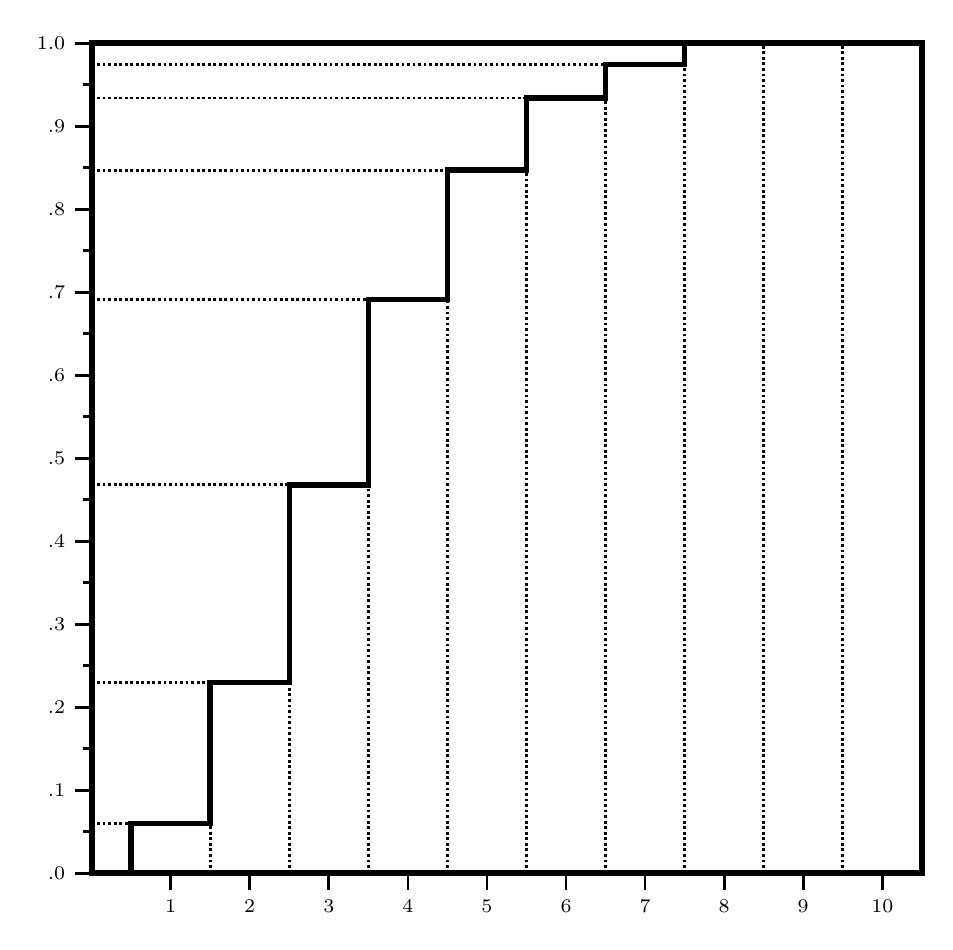
\begin{tikzpicture}
      \begin{axis}[
        width=1\textwidth,
        height=1\textwidth,
        ymin=0,
        ymax=1.0,
        xmin=0.5,
        xmax=11.0,
        ytick={0.0,0.1,0.2,0.3,0.4,0.5,0.6,0.7,0.8,0.9,1.0},
        yticklabels={\axisfont .0,\axisfont .1,\axisfont .2,\axisfont .3,\axisfont .4,\axisfont .5,\axisfont .6,\axisfont .7,\axisfont .8,\axisfont .9,\axisfont 1.0},
        xtick={1.5,2.5,3.5,4.5,5.5,6.5,7.5,8.5,9.5,10.5},
        xticklabels={\axisfont 1,\axisfont 2,\axisfont 3,\axisfont 4,\axisfont 5,\axisfont 6,\axisfont 7,\axisfont 8,\axisfont 9,\axisfont 10},
        axis lines=box,
        axis line style={line width=2.2pt},
        tick style={black,line width=1pt},
        major tick length=6pt,
        minor tick length=3pt,
        minor y tick num=1,
        tick align=outside,
        xtick pos=left,
        ytick pos=left,
        tick label style={font=\axisfont\scriptsize,/pgf/number format/assume math mode=false},
        xticklabel style={font=\axisfont\scriptsize,/pgf/number format/assume math mode=false},
        yticklabel style={font=\axisfont\scriptsize,/pgf/number format/assume math mode=false},
        enlargelimits=false,
        xmajorgrids=false,
        ymajorgrids=false,
        grid style={dotted, line width=0.6pt},
      ]
        % Figure 1.2 box: short horizontal dotted connectors from y-axis.
        \addplot[densely dotted, line width=1pt, forget plot] coordinates {(0.5,0.060) (1.0,0.060)};
        \addplot[densely dotted, line width=1pt, forget plot] coordinates {(0.5,0.230) (2.0,0.230)};
        \addplot[densely dotted, line width=1pt, forget plot] coordinates {(0.5,0.468) (3.0,0.468)};
        \addplot[densely dotted, line width=1pt, forget plot] coordinates {(0.5,0.691) (4.0,0.691)};
        \addplot[densely dotted, line width=1pt, forget plot] coordinates {(0.5,0.847) (5.0,0.847)};
        \addplot[densely dotted, line width=1pt, forget plot] coordinates {(0.5,0.934) (6.0,0.934)};
        \addplot[densely dotted, line width=1pt, forget plot] coordinates {(0.5,0.974) (7.0,0.974)};
        % Figure 1.2 box: step function (cumulative).
        \addplot[const plot,line width=2pt]
          coordinates {
            (0,0)
            (1,0.060)
            (2,0.230)
            (3,0.468)
            (4,0.691)
            (5,0.847)
            (6,0.934)
            (7,0.974)
            (8,1.000)
            (9,1.000)
            (10,1.000)
          };
        % Figure 1.2 box: vertical dotted guides at each integer.
        \addplot[densely dotted,line width=1pt] coordinates {(1,0) (1,0.060)};
        \addplot[densely dotted,line width=1pt] coordinates {(2,0) (2,0.060)};
        \addplot[densely dotted,line width=1pt] coordinates {(3,0) (3,0.230)};
        \addplot[densely dotted,line width=1pt] coordinates {(4,0) (4,0.468)};
        \addplot[densely dotted,line width=1pt] coordinates {(5,0) (5,0.691)};
        \addplot[densely dotted,line width=1pt] coordinates {(6,0) (6,0.847)};
        \addplot[densely dotted,line width=1pt] coordinates {(7,0) (7,0.934)};
        \addplot[densely dotted,line width=1pt] coordinates {(8,0) (8,1.000)};
        \addplot[densely dotted,line width=1pt] coordinates {(9,0) (9,1.000)};
        \addplot[densely dotted,line width=1pt] coordinates {(10,0) (10,1.000)};
      \end{axis}
    \end{tikzpicture}
  \end{minipage}
  \caption{Sampling the File Length Distribution}
  \label{fig:sample-file-length}
\end{figure}
